\documentclass[11pt,draftcls,onecolumn,peerreview]{IEEEtran}
\bibliographystyle{plain}
\usepackage{graphicx}
\usepackage{amssymb}
\usepackage{amsmath}
\usepackage[bbgreekl]{mathbbol}
\DeclareMathOperator*{\argmax}{argmax}
\DeclareMathOperator*{\argmin}{argmin}
\usepackage[affil-it]{authblk}
\usepackage{paralist}
\usepackage{url}
\usepackage{tabularx}
\usepackage{color}
\usepackage{tikz}
\usepackage{tipa}\newcommand{\ipa}[1]{\textipa{#1}}
\usepackage{stackrel}
\usetikzlibrary{positioning,shadows,arrows,shapes,calc}
\setlength{\textwidth}{6.5in}
\setlength{\textheight}{9in}
\setlength{\oddsidemargin}{0in}
\setlength{\topmargin}{0in}
\newcommand{\mytikzscale}{1.0}

\title{ASR for Under-Resourced Languages from Probabilistic Transcription}

\author{Mark Hasegawa-Johnson$^1$,~\IEEEmembership{Senior~Member,~IEEE}
  Preethi Jyothi$^1$,~\IEEEmembership{Member,~IEEE}
  Daniel McCloy$^2$,
  Majid Mirbagheri$^2$,
  Giovanni di Liberto$^3$,
  Amit Das$^1$,~\IEEEmembership{Student~Member,~IEEE}
  Bradley Ekin$^2$,~\IEEEmembership{Student~Member,~IEEE}
  Chunxi Liu$^4$,
  Vimal Manohar$^4$,~\IEEEmembership{Student~Member,~IEEE}
  Hao Tang$^5$,
  Edmund C. Lalor$^3$,
  Nancy F.\ Chen$^6$,~\IEEEmembership{Senior~Member,~IEEE}
  Paul Hager$^7$,
  Tyler Kekona$^2$,
  Rose Sloan$^8$,
  and Adrian KC Lee$^2$~\IEEEmembership{Member,~IEEE}
}
\affil{1. University of Illinois, 2. University of Washington,
  3. Trinity College, Dublin, 4. Johns Hopkins University, 5. Toyota
  Technological Institute Chicago, 6. Institute for Infocomm Research,
  7. MIT, 8. Yale University}

\markboth{Draft, for review only}
{Hasegawa-Johnson \MakeLowercase{\textit{et al.}}: ASR for Under-Resourced Languages from Probabilistic Transcription}

\begin{document}
\maketitle

\begin{abstract}
\input{s0_abstract.tex}
\end{abstract}

\begin{IEEEkeywords}
Automatic speech recognition, Under-resourced languages, Mismatched crowdsourcing, EEG
\end{IEEEkeywords}

\ifCLASSOPTIONpeerreview
\begin{center} \bfseries EDICS Category: SPE-RECO \end{center}
\fi
% For peerreview papers, this IEEEtran command inserts a page break and
% creates the second title. It will be ignored for other modes.
\IEEEpeerreviewmaketitle

%%%%%%%%%%%%%%%%%%%%%%%%%%%%%%%%%%%%%%%%%%%
\section{Introduction}

\IEEEPARstart{A}{utomatic} speech recognition (ASR) has the potential to provide
database access, simultaneous translation, and text/voice messaging
services to anybody, in any language, dramatically reducing linguistic
barriers to economic success.  To date, ASR has failed to achieve its
potential, because successful ASR requires very large labeled
corpora. Current methods require about 1000 hours of transcribed
speech per language, transcribed at a cost of about 6000 hours of
human labor; the human transcribers must be computer-literate, and
they must be native speakers of the language being transcribed.
%In
%many languages, recruiting dozens of computer-literate
%native speakers is impractical.
{\color{blue} Doing so is beyond the resources of most under-resourced language
communities; we have found that transcribing even one hour of speech
is beyond the reach of some under-resourced language communities.
In order to create the databases reported in this paper, we sought
paid native transcribers for the seventy languages in which we have
untranscribed audio data.  We found transcribers willing to work in
only eleven of those languages, of which only seven finished the task.}

Instead of recruiting native transcribers in search of a perfect
reference transcript, this paper proposes the use of probabilistic
transcripts.  A probabilistic transcript is a probability mass
function, $\rho_\Phi(\phi)$, specifying, as a real number between $0$ and
$1$, the probability that any particular phonetic transcript $\phi$
is the correct transcript of the utterance.  Prior to this work,
machine learning has almost always assumed that the training dataset
contains either deterministic transcripts
($\rho_{DT}(\phi)\in\left\{0,1\right\}$, commonly called ``supervised
training'') or completely untranscribed utterances (commonly called
``unsupervised training,'' in which case we assume that $\rho_{LM}(\phi)$
is given by some {\em a priori} language model).  This article
proposes that, even in the absence of a deterministic transcript,
there may be auxiliary sources of information that can be compiled to
create a probabilistic transcript with entropy lower than that
of the language model, and that machine learning methods applied to
the probabilistic transcript are able to make use of its reduced
entropy in order to learn a better ASR.  In particular,
this paper considers three useful auxiliary sources of information:
\begin{enumerate}
\item SELF-TRAINING: ASR pre-trained in other languages is used to
  transcribe unlabeled training data in the target language.
\item MISMATCHED CROWDSOURCING: Human crowd workers who don't speak
  the target language are asked to transcribe it as if it were a
  sequence of nonsense syllables.
\item EEG DISTRIBUTION CODING: Humans who do not speak the target
  language are asked to listen to its extracted syllables, and their
  EEG responses are interpreted as a probability mass function over
  possible phonetic transcripts.
\end{enumerate}



%%%%%%%%%%%%%%%%%%%%%%%%%%%%%%%%%%%%%%%%%%%%%%%%%%%%%%%%%%%%%%
\section{Background}

Suppose we require that, in
order to develop speech technology, it is necessary first to have (1)
some amount of recorded speech audio, and (2) some amount of text
written in the target language.  These two requirements can be met by
at least several hundred languages: speech audio can be recorded
from podcasts or radio broadcasts,
and text can be acquired from Wikipedia, Bibles, and textbooks.
Recorded speech is, however, not usually transcribed; and the
requirement of native language transcription is beyond the economic
capabilities of many minority-language communities.

\subsection{ASR in Under-Resourced Languages}

Krauwer~\cite{Krauwer2003} defined an under-resourced language to be
one that lacks: stable orthography, significant
presence on the internet, linguistic expertise, monolingual tagged
corpora, bilingual electronic dictionaries, transcribed speech,
pronunciation dictionaries, or other similar electronic resources.
Berment~\cite{Berment2004} defined a rubric for tabulating the
resources available in any given language, and proposed that a
language should be called ``under-resourced'' if it scored lower than
10.0/20.0 on the proposed rubric.  By these standards, technology
for under-resourced languages is most often demonstrated on
languages that are not really under-resourced: for example, ASR may be
trained without transcribed speech, but the quality of the resulting
ASR can only be proven by measuring its phone error
rate (PER) or word error rate (WER) using transcribed speech.  The
intention, in most cases, is to create methods that can later be
ported to truly under-resourced languages.

The International Phonetic Alphabet (IPA~\cite{ipa1993}) is a set of
symbols representing speech sounds (phones) defined by the principle
that, if two phones are used contrastively
 (i.e., they represent distinct phonemes) in any language, then
those phones should have distinct symbolic representations in the IPA.
This makes the IPA a natural choice for transcripts used to train
cross-language ASR systems, and indeed ASR in a new language can be 
rapidly deployed using acoustic models trained to represent every 
distinct symbol in the IPA~\cite{Schultz2001}.
However, because IPA symbols are defined phonemically, there is no
guarantee of cross-language equivalence in the acoustic properties of
the phones they represent. This problem arises even between dialects of
the same language: a monolingual Gaussian mixture model (GMM) trained on
five hours of Levantine Arabic can be improved by adding ten hours of
Standard Arabic data, but only if the log likelihood of cross-dialect
data is scaled by 0.02~\cite{Huang2012}.

Better cross-language transfer of acoustic models can be achieved, but
only by using structured transfer learning methods, including neural
networks (NN) and subspace Gaussian mixture models (SGMM).  SGMMs use
language-dependent GMMs, each of which is the linear interpolation of
language-independent mean and variance vectors~\cite{Povey2011}, e.g.,
16\% relative WER reduction was achieved in Tamil by combining SGMM
with an acoustic data normalization technique~\cite{Mohan2014}.  NN
transfer learning can be categorized as tandem, bottleneck,
pre-training, phone mapping, and multi-softmax methods.  In a tandem
system, outputs of the NN are Gaussianized, and used as features whose
likelihood is computed with a GMM; in a
bottleneck system, features are extracted from a hidden layer rather
than the output layer. Both tandem~\cite{Stolcke2006} and
bottleneck~\cite{Vesely2012} features trained on other languages can
be combined with GMMs~\cite{Vesely2012} or SGMMs~\cite{Imseng2014}
trained on the target language in order to improve WER.

A hybrid ASR is a system in which the NN terminates in a softmax
layer, whose outputs are interpreted as phone or
senone~\cite{Dahl2012} probabilities.  Knowledge of the target
language phone inventory is necessary to train a hybrid ASR, but it is
possible to reduce WER by first pre-training the NN hidden layers with
multilingual data~\cite{Huang2013,Swietojanski2012}.  A hybrid ASR can be
constructed using very little in-language speech data by adding a
single phone-mapping layer~\cite{Sim2008} or senone-mapping layer~\cite{Do2012}
to the output of the multilingual NN.  A multi-softmax system
is a network with several different language-dependent softmax
layers, each of which is the linear transform of a multilingual shared
hidden layer~\cite{Huang2013,Scanzio2008,Vesely2012}.

\subsection{Self-Training}

Self-training is a class of semi-supervised learning techniques in
which a classifier labels unlabeled data, and is then
re-trained using its own labels as targets.  Self-training is
frequently used to adapt ASR from a well-resourced language to an
under-resourced language~\cite{Loof2009,Cetin2008}, or in some cases,
to create target-language ASR by adapting several source-language
ASRs~\cite{Vu2011b}.  A self-trained classifier tends to be too
conservative, because the tails of the data distribution are truncated
by the self-labeling process~\cite{Scudder1965}; on the other hand, a
self-trained classifier needs to be conservative, because the error
rate of the learned classifier increases at a rate more than
proportional to the error rate of the self-labeling
process~\cite{Huang2013b}.  Self-training is therefore most useful
when the in-language training data are filtered, to exclude
frames with confidence below a threshold~\cite{vesely2013-semi},
and/or weighted, so that some frames are allowed to influence the
learned parameters more than others~\cite{Hsiao2013}.  Self-training
of NN systems has been shown to be about 50\% more effective (1.5
times the error rate reduction) as self-training of GMM
systems~\cite{Huang2013b}.

\subsection{Mismatched Crowdsourcing}
\label{sec:bgmc}

\begin{figure}[b!]\setlength{\textfloatsep}{3mm}
\begin{center}
  \tikzstyle{pre2}=[<-,>=stealth',thick, draw=black]
  \tikzstyle{post2}=[->,>=stealth',thick, draw=black]
  \begin{tikzpicture}[
      scale=\mytikzscale,
      boxed/.style={rectangle,thick, draw=black, text=black, rounded corners=1mm, text centered, text width=2.5cm},
      open/.style={text=black, text centered, text width=3cm},
      every node/.style={transform shape}      
    ]
    \node[open] (n0) at (-4.5,1) {\large $w=$Utterance-language words\\\vspace*{0.1in}$<$$\vcenter{\hbox{\includegraphics[width=1in]{../figs/vaakpahachaan.png}}}$$>$};
    \node[boxed] (n1) at (-0.75,1) {\large Human talker modeled by a pronunciation FST,\\$\rho(\phi|w)$} 
    edge[pre2](n0);
    \node[boxed] (n2) at (2.5,1) {\large Human listener modeled by a misperception FST,\\$\rho(\psi|\phi)$}
    edge[pre2] (n1);
    \node[boxed] (n3) at (5.75,1) {\large Human transcriber modeled as a phoneme-to-grapheme FST, $\rho(\lambda|\psi)$}
    edge[pre2] (n2);
    \node[open] (n4) at (9,1) {\large $\lambda$: Annotation-language orthography\\$<$vak paychan$>$} 
    edge[pre2](n3);
    \node[open] (n5) at (1,-1.5) {\large $\phi=$Utterance phones\\\ipa{[va:k p@H@tSa:n]}};
    \node[open] (n6) at (4,-1.5) {\large $\psi=$Perceived phones\\\ipa{[vAk p\textsuperscript{h}eItSAn]}}; 
  \end{tikzpicture}\\
\end{center}
\setlength{\abovecaptionskip}{0pt}
\caption{Mismatched Crowdsourcing: crowd workers on the web are asked
  to transcribe speech in a language they do not know.  Annotation
  mistakes are modeled by a finite state transducer (FST) model of
  utterance-language pronunciation variability (reduction and
  coarticulation), composed with an FST model of non-native speech
  misperception (mapping utterance-language phones to
  annotation-language phones), composed with an inverted
  grapheme-to-phoneme (G2P) transducer.}
\label{fig:h2e_eg2}
\end{figure}

In~\cite{JHJ15a}, a methodology was proposed that bypasses the need
for native language transcription: mismatched crowdsourcing sends target
language speech to crowd-worker transcribers who have no
knowledge of the target language, then uses explicit mathematical
models of second language phonetic perception to recover an equivalent
phonetic transcript (Fig.~\ref{fig:h2e_eg2}).  Majority voting is
re-cast, in this paradigm, as a form of error-correcting code
(redundancy coding), which effectively increases the capacity of the
noisy channel; interpretation as a noisy channel permits us to explore
more effective and efficient forms of error-correcting codes.
Assume that cross-language phone misperception is a finite-memory
process, and can therefore be modeled by a finite state transducer
(FST).  The complete sequence of representations from utterance
language to annotation language can therefore be modeled as a noisy
channel represented by the composition of up to three consecutive FSTs
(Fig.~\ref{fig:h2e_eg2}): a pronunciation model, a misperception
model, and an inverted grapheme-to-phoneme (G2P) transducer.

\subsection{Electrophysiology of Speech Perception}

The human auditory system is sensitive to within-category distinctions
in speech sounds, but such pre-categorical perceptual distinctions may
be lost in transcription tasks, where a listener must filter their
percepts through the limited number of categorical representations
available in their native language orthography.  EEG distribution
coding is a proposed new method that interprets the electrical evoked
potentials of an untrained listener (measured by
electroencephalography or EEG) as a probability distribution
over the phone set of the utterance language
(Fig.~\ref{fig:eeg_paradigm}).  A transcriber, in this scenario, listens
to speech in both his native language and an unfamiliar non-native
target language, while his EEG responses are recorded.  From his
responses to English speech, an English-language EEG phone recognizer
is trained~\cite{Liberto15}.  Misperception probabilities
$\rho(\psi|\phi)$ are then estimated: for each non-native phone
$\phi$, the classifier outputs are interpreted as an estimate of
$\rho(\psi|\phi)$.

\begin{figure}\setlength{\textfloatsep}{3mm}
\setlength{\fboxsep}{0pt}%
\setlength{\fboxrule}{0.5pt}%
\begin{center}
  \begin{tikzpicture}[
      scale=\mytikzscale,
      boxed/.style={rectangle,thick, draw=black, text=black, fill=white, 
      	rounded corners=1mm, text centered, text width=2.5cm},
      every node/.style={transform shape}      
    ]
    \node[text width=1.5in, text centered, anchor=north] (label0) at (-5,2.75) {\large EEG response to foreign phones (epoched \& averaged)};
    \node[text width=2.5in, text centered, anchor=north] (label1) at (0,2.75) {\large EEG feature classifiers trained on feature-labeled English phones};
    \node (raweeg) at (-5,0) {\fbox{\includegraphics[width=1in]{../figs/avg-eeg.pdf}}};
    \node[boxed] (f0) at (-0.4,1.1) {\large\phantom{pd}};
    \node[boxed] (f1) at (-0.3,0.9) {\large\phantom{pd}};
    \node[boxed] (f2) at (-0.2,0.7) {\large\phantom{pd}};
    \node[boxed] (f3) at (-0.1,0.5) {\large\phantom{pd}};
    \node[boxed] (f4) at (0.0,0.3) {\large\phantom{pd}};
    \node[boxed] (f5) at (0.15,0.1) {\large\phantom{p}continuant\phantom{d}};
    \node[boxed] (f6) at (0.45,-0.4) {\large\phantom{p}sonorant\phantom{d}};
    \node[boxed] (f7) at (0.75,-0.9) {\large aspirated};
    \draw[->, thick] (-3.25,0) -- (-2,0);
    \draw[->, thick] (2,0) -- (3,0);
    \node[text width=1in, text centered] (label2) at (4.5,0) {\large \baselineskip=8pt Foreign phone misperception probabilities};
  \end{tikzpicture}\\
\end{center}
\setlength{\abovecaptionskip}{0pt}
  \caption{EEG responses are recorded while the listener hears speech in
    his native language.  A bank of distinctive
    feature classifiers are trained.  The listener then hears speech in an
    unfamiliar language, and his EEG responses are classified,
    in order to estimate arc weights in the misperception FST.}
  \label{fig:eeg_paradigm}
\end{figure}


%%%%%%%%%%%%%%%%%%%%%%%%%%%%%%%%%%%%%%%%%%%%%%%%
\section{Algorithms that Induce a Probabilistic Transcript}

A deterministic transcript is a sequence of phone symbols,
$\phi^\ell =[\phi_1^\ell,\ldots,\phi_M^\ell]$ where $\phi_m^\ell$ is a
symbol drawn from the phone set of the utterance language.

A probabilistic transcript is a probability mass function (pmf)
over the set of deterministic transcripts.  Capital letters denote
random variables, lowercase denote instances: $\Phi^{\ell}_m$ is a
random variable whose instance is $\phi_m^\ell$.
Denote the probability of transcript $\phi^{\ell}$
as $\rho_{\Phi^\ell}(\phi^{\ell})$, where $\rho$ (``reference'') means
that $\rho_{\Phi^\ell}(\phi^{\ell})$ is a reference distribution---a
distribution specified by the probabilistic transcription process, and
not dependent on ASR parameters during training.  The
distribution label $\Phi^\ell$ is omitted when clear from the instance
label, e.g., $\rho(\phi^\ell)$, but $\rho_{\Phi^\ell}(u)$.
Superscript denotes waveform index, while subscript denotes frame or
phone index.  Absence of either superscript or subscript denotes a
collection, thus $\Phi=\left\{\Phi^1,\ldots,\Phi^L\right\}$ (with
instance value $\phi=\left\{\phi^1,\ldots,\phi^L\right\}$) is the
random variable over all transcripts of the database.  In all of
the work described in this paper, the probabilistic transcript is
represented as a confusion network~\cite{Mangu00}, meaning that it is
the product of independent symbol pmfs $\rho(\phi_m^\ell)$:
\begin{equation}
  \rho(\phi)=\prod_{\ell=1}^L\rho(\phi^\ell)=
  \prod_{\ell=1}^L \prod_{m=1}^M \rho(\phi_m^{\ell})
\end{equation}
The pmf $\rho(\phi^\ell)$ can be represented as a weighted
finite state transducer (wFST) in which edges connect states in a
strictly left-to-right fashion without skips, and in which the edges
connecting state $m$ to state $m+1$ are weighted according to the pmf
$\rho(\phi_m^\ell)$ (Fig.~\ref{fig:pt}).
\begin{figure}
\begin{center}
  \tikzstyle{pre}=[<-,shorten <=1pt,>=stealth',semithick,draw=black]
  \tikzstyle{post}=[->,shorten >=1pt,>=stealth',semithick,draw=black]
  \begin{tikzpicture}[
      scale=\mytikzscale,
      state/.style={circle,thick, draw=black, text=black, text width=0.25cm},
      every node/.style={transform shape}
    ]
    \node[state] (g0) at (0,0) {};
    \node[state] (g1) at (2,0) {};
    \draw[post] (g0) -- (0.5,1) -- (1.5,1) -- (g1);
    \node at (1,1.25) {\large\ipa{[a]}$/0.5$};
    \draw[post] (g0) -- (0.5,0) -- (1.5,0) -- (g1);
    \node at (1,0.25) {\large\ipa{[\ae]}$/0.4$};
    \draw[post] (g0) -- (0.5,-1) -- (1.5,-1) -- (g1);
    \node at (1,-0.75) {\large$\emptyset/0.1$};
    \node[state] (g2) at (4,0) {};
    \draw[post] (g1) -- (2.5,1.5) -- (3.5,1.5) -- (g2);
    \node at (3,1.75) {\large\ipa{[b\super{H}]}$/0.45$};
    \draw[post] (g1) -- (2.5,0.5) -- (3.5,0.5) -- (g2);
    \node at (3,0.75) {\large\ipa{[V]}$/0.35$};
    \draw[post] (g1) -- (2.5,-0.5) -- (3.5,-0.5) -- (g2);
    \node at (3,-0.25) {\large\ipa{[b]}$/0.10$};
    \draw[post] (g1) -- (2.5,-1.5) -- (3.5,-1.5) -- (g2);
    \node at (3,-1.25) {\large\ipa{[p]}$/0.10$};
    \node[state] (g3) at (6,0) {};
    \draw[post] (g2) -- (4.5,1) -- (5.5,1) -- (g3);
    \node at (5,1.25) {\large\ipa{[i]}$/0.7$};
    \draw[post] (g2) -- (4.5,0) -- (5.5,0) -- (g3);
    \node at (5,0.25) {\large\ipa{[e]}$/0.2$};
    \draw[post] (g2) -- (4.5,-1) -- (5.5,-1) -- (g3);
    \node at (5,-0.75) {\large$\emptyset/0.1$};
    \node[state] (g4) at (8,0) {};
    \draw[post] (g3) -- (6.5,1.5) -- (7.5,1.5) -- (g4);
    \node at (7,1.75) {\large\ipa{[a]}$/0.3$};
    \draw[post] (g3) -- (6.5,0.5) -- (7.5,0.5) -- (g4);
    \node at (7,0.75) {\large\ipa{[\ae]}$/0.3$};
    \draw[post] (g3) -- (6.5,-0.5) -- (7.5,-0.5) -- (g4);
    \node at (7,-0.25) {\large\ipa{[i]}$/0.2$};
    \draw[post] (g3) -- (6.5,-1.5) -- (7.5,-1.5) -- (g4);
    \node at (7,-1.25) {\large\ipa{[e]}$/0.2$};
    \node[state] (g5) at (10,0) {};
    \draw[post] (g4) -- (8.5,1) -- (9.5,1) -- (g5);
    \node at (9,1.25) {\large\ipa{[m]}$/0.6$};
    \draw[post] (g4) -- (8.5,0) -- (9.5,0) -- (g5);
    \node at (9,0.25) {\large\ipa{[n]}$/0.2$};
    \draw[post] (g4) -- (8.5,-1) -- (9.5,-1) -- (g5);
    \node at (9,-0.75) {\large\ipa{[N]}$/0.2$};
    \node[state] (g6) at (12,0) {};
    \draw[post] (g5) -- (10.5,1) -- (11.5,1) -- (g6);
    \node at (11,1.25) {\large\ipa{[i]}$/0.4$};
    \draw[post] (g5) -- (10.5,0) -- (11.5,0) -- (g6);
    \node at (11,0.25) {\large\ipa{[e]}$/0.4$};
    \draw[post] (g5) -- (10.5,-1) -- (11.5,-1) -- (g6);
    \node at (11,-0.75) {\large$\emptyset/0.2$};
    \node[state] (g7) at (14,0) {};
    \draw[post] (g6) -- (12.5,1.5) -- (13.5,1.5) -- (g7);
    \node at (13,1.75) {\large\ipa{[k]}$/0.4$};
    \draw[post] (g6) -- (12.5,0.5) -- (13.5,0.5) -- (g7);
    \node at (13,0.75) {\large\ipa{[k\super h]}$/0.3$};
    \draw[post] (g6) -- (12.5,-0.5) -- (13.5,-0.5) -- (g7);
    \node at (13,-0.25) {\large\ipa{[g\super{H}]}$/0.1$};
    \draw[post] (g6) -- (12.5,-1.5) -- (13.5,-1.5) -- (g7);
    \node at (13,-1.25) {\large\ipa{[g]}$/0.1$};
    \draw[post] (g6) -- (12.5,-2.5) -- (13.5,-2.5) -- (g7);
    \node at (13,-2.25) {\large$\emptyset/0.1$};
  \end{tikzpicture}
\end{center}
\vspace*{-2mm}
\caption{A probabilistic transcript (PT) is a probability mass
  function (pmf) over candidate phonetic transcripts.  All PTs
  considered in this paper can be expressed as confusion networks,
  thus, as sequential pmfs over the null-augmented space of IPA
  symbols.  In this schematic example, $\emptyset$ is the null
  symbol, symbols in brackets are IPA, and numbers indicate
  probabilities.}
  \label{fig:pt}
\end{figure}

Three different experimental sources were tested for the creation of a
PT.  Self-training is now well-established in the field of
under-resourced ASR; we adopted the algorithm of Vesely, Hannemann and
Burget~\cite{vesely2013-semi}.  Mismatched crowdsourcing used original
annotations collected using published methods~\cite{JHJ15b}.  EEG was
not used independently here, but rather, was used to learn a
misperception model applicable to the interpretation of mismatched
crowdsourcing.

\subsection{Self-Training}
\label{sec:selftraining}

The first set of PTs is computed using NN self-training.
The Kaldi toolkit~\cite{Kaldi2011} is first used to train a
cross-lingual baseline ASR, using training data drawn from six
languages not including the target language.  The goal of
self-training, then, is to adapt the NN to a database containing
$L$ speech waveforms in the target language, each represented by
acoustic feature matrix $x^\ell =[x_1^\ell,\ldots,x_T^\ell]$, where
$x_t^\ell$ is an acoustic feature vector.  The feature matrix $x^\ell$
represents an utterance of an unknown phone transcript
$\phi^\ell=[\phi_1^\ell,\ldots,\phi_M^\ell]$ which, if known, would
determine the sequence but not the durations of senones (HMM states)
$s^\ell =[s_1^\ell,\ldots,s_T^\ell]$.

The feature matrix $x^\ell$ is decoded using the cross-lingual
baseline ASR, generating a phone lattice output.  Using scripts
provided by previous experiments~\cite{vesely2013-semi}, the phone
lattice is interpreted as a set of posterior senone probabilities
$\rho(s_t^\ell|x_t^\ell)$ for each frame, and the senone posteriors
serve as targets for re-estimating the NN weights.
Experiments using other datasets found that self-training
should use best-path alignment to specify a binary target for NN
training~\cite{vesely2013-semi}, but, apparently because of
differences in the adaptation set between our experiments and previous
work, we achieve better performance using real-valued targets.
{\color{blue} As in previous work, senones with a posterior probability
  below 0.7 were removed from the training set, thus the training target
  was a number between 0.7 and 1.0.}

\subsection{Mismatched Crowdsourcing}
\label{sec:MC}

\begin{figure}[b!]\setlength{\textfloatsep}{3mm}
\begin{center}
  \tikzstyle{pre}=[<-,shorten <=3pt,>=stealth',thick, draw=black]
  \tikzstyle{post}=[->,shorten >=3pt,>=stealth',thick, draw=black]
  \begin{tikzpicture}[
      scale=\mytikzscale,
      boxed/.style={rectangle,thick, draw=black, text=black, rounded corners=1mm, text centered, text width=5cm},
      state/.style={circle,thick, draw=black, text=black, text width=0.25cm},
      open/.style={text=black, text centered},
      every node/.style={transform shape}
    ]
    \node[open] (n0) at (1,0) {\begin{tabular}{c}$T$=Mismatched\\Transcripts\\\hline trabiza\\ta peesome\\ta pisha\\chah peesh um\\shapisha\\sabeesham\\chapiser\\some pizza\end{tabular}};
    \node[boxed] (n1) at (6,0) {\begin{tabular}{c}$\rho(\lambda|T)$\\\hline\vspace{3cm}\end{tabular}} edge[pre] (n0);
    \node[state] (g0) at (4,-0.25) {};
    \node[state] (g1) at (6,-0.25) {};
    \node (g2) at (8,-0.25) {\ldots};
    \draw[post] (g0) -- (4.25,0.75) -- (5.75,0.75) -- (g1);
    \node at (5,1) {$<$t$>$$/0.4$};
    \draw[post] (g0) -- (g1);
    \node at (5,0) {$<$ch$>$$/0.4$};
    \draw[post] (g0) -- (4.25,-1.25) -- (5.75,-1.25) -- (g1);
    \node at (5,-1) {$<$s$>$$/0.2$};
    \draw[post] (g1) -- (g2);
    \node at (7,0) {$<$a$>$$/1.0$};
    \node[boxed] (n2) at (12,0) {\begin{tabular}{c}$\rho(\phi|T)$\\\hline\vspace*{3cm}\end{tabular}} edge[pre] (n1);
    \node[state] (g10) at (10,-0.25) {};
    \node[state] (g11) at (12,-0.25) {};
    \node (g12) at (14,-0.25) {\ldots};
    \draw[post] (g10) -- (10.25,0.75) -- (11.75,0.75) -- (g11);
    \node at (11,1) {\ipa{[t]}$/0.4$};
    \draw[post] (g10) -- (g11);
    \node at (11,0) {\ipa{[tS]}$/0.4$};
    \draw[post] (g10) -- (10.25,-1.25) -- (11.75,-1.25) -- (g11);
    \node at (11,-1) {\ipa{[s]}$/0.2$};
    \draw[post] (g11) -- (g12);
    \node at (13,0) {\ipa{[A]}$/1.0$};
  \end{tikzpicture}\\
\end{center}
\setlength{\abovecaptionskip}{0pt}
\caption{Probabilistic transcription from mismatched crowdsourcing:
  Transcripts $T$ are filtered to remove outliers, and merged to
  create a confusion network over orthographic symbols,
  $\rho(\lambda|T)$, from which the probabilistic transcript
  $\rho(\phi|T)$ is inferred. Example shown: Swahili speech,
  English-speaking transcribers.  Symbols in $<$$>$ are graphemes,
  symbols in $[]$ are phones, numbers are probabilities.}
\label{fig:mcmethods}
\end{figure}

The second set of PTs was computed by sending audio in the target
language to non-speakers of the target language, and asking them to
write what they hear.  It would be preferable to recruit transcribers
who speak a language with predictable orthography, but since
transcribers in those languages were more expensive, this
experiment instead recruited transcribers who speak American English.
Denote using $T$ the set of mismatched
transcripts produced by these English-speaking crowd workers,
which we wish to interpret as a pmf over
target-language phone sequences, $\rho(\phi|T)$.  As an intermediate
step, prior work~\cite{JHJ15b} developed techniques
to merge texts into a confusion network
$\rho(\lambda|T)$ over representative transcripts in the
annotation-language orthography (Fig.~\ref{fig:mcmethods}).
%Formation of
%$\rho(\lambda|T)$ involves data filtering to remove outliers (based on
%pair-wise string edit distance among transcripts), expansion of the
%orthography to an alphabet that includes
%single-character symbols for digraphs and sequences commonly used to represent
%single phonemes in English orthography ($<$ai, ay, ee, oo, ou, aw, ow,
%bh, ch, dh, gh, jh, kh, ph, sh, th, wh, zh, ck$>$, and any vowel followed by
%a word-final silent $<$e$>$), and a weighted
%voting scheme in which the weight of each transcript is proportional
%to the frequency with which it matches the other transcripts.

Once transcripts have
been aligned and filtered to create the orthographic confusion network
$\rho(\lambda|T)$, they are then translated into a distribution over
phone transcripts according to:
\begin{align}
  \rho(\phi|T) 
%  &=\sum_{\lambda} \rho(\phi|\lambda,T) \rho(\lambda|T) \notag \\
  &\approx \max_{\lambda}  \rho(\phi|\lambda) \rho(\lambda|T) \notag \\
  &= \max_{\lambda}  \left(\frac{\rho(\lambda|\phi)}{\rho(\lambda)}
  \rho(\phi)\right) \rho(\lambda|T) 
\label{eq:PT}
\end{align}
The terms other than $\rho(\lambda|T)$ in Equation~(\ref{eq:PT}) are
estimated as follows.  $\rho(\lambda)$ is modeled using a unigram
prior over the letter sequences in $\lambda$.  $\rho(\phi)$ is modeled
using {\color{blue} either a cross-lingual phone unigram, a
  language-specific phone zero-gram (the cross-lingual unigram,
  constrained to take values from the phone set of the target
  language), or a language-specific phone bigram
  $\rho(\phi)=\prod_{m=1}^M \rho(\phi_m|\phi_{m-1})$.
  Sec.~\ref{sec:trainwithlm} compares the results of these three
  methods, and describes how the phone bigram was trained.}
%, trained
%on a corpus of Wikipedia text in the target language, converted into
%phone sequences as described in Section~\ref{sec:trainwithlm}.
$\rho(\lambda|\phi)$ is called the misperception G2P, as it maps to
graphemes in the annotation language, $\lambda$, from phones in the
utterance language, $\phi$.  Section~\ref{sec:eegchanmod} describes
methods that decompose $\rho(\lambda|\phi)$ into separate
misperception and G2P transducers, but it can also be trained directly
using
%the Carmel toolkit \cite{Knight99} as an FST mapping phones to letters
%based on
representative transcripts $\lambda$ (and their
corresponding native transcripts) for speech {\em in languages other
  than the target language}.
{\color{blue} The model learned in this way is essentially
  a machine translation model, which translates between graphemes in
  the annotation language ($\lambda$) to phonemes in any possible
  utterance language ($\phi$).}
%Sec.~\ref{sec:mlbaseline}
% of this article uses
%  a similar method, though without left and right context, to map
%  training phonemes to test phonemes in a self-trained neural network.}
We assume that misperceptions depend more
heavily on the annotation language than on the utterance language, and
that therefore a model $\rho(\lambda|\phi)$ trained using a universal
phone set for $\phi$ is also a good model of $\rho(\lambda|\phi)$ for
the target language. Note that, while this assumption is not entirely
accurate, it is necessitated by the requirement that no native
transcripts in the target language can be used in building any part
of our system.
%We also allow this FST to delete phones and insert letters.


\subsection{Estimating Misperceptions from Electrocortical Responses}
\label{sec:eegchanmod}

The misperception G2P described in Section~\ref{sec:MC} was estimated
using a combination of mismatched and deterministic transcripts of
non-target languages. However, with a small amount
of transcribed data in the utterance language, it is possible
to estimate the misperception G2P using electrocortical measurements
of non-native speech perception. In this approach, the misperception G2P
is decomposed into two separate transducers,
a misperception transducer $\rho(\psi|\phi)$, and an
annotation-language G2P $\rho(\lambda|\psi)$:
\begin{equation}
  \rho(\lambda|\phi)\approx\sum_{\psi}\rho(\lambda|\psi)\rho(\psi|\phi)
\end{equation}
where $\phi$ is a phone string in the utterance language, $\psi$ is a
phone string in the annotation language, and $\lambda$ is an
orthographic string in the annotation language.  $\rho(\lambda|\psi)$
is an inverted G2P in the annotation language, e.g., trained on the
CMU dictionary of American English pronunciations~\cite{Lenzo1995}.
$\rho(\psi|\phi)$ is the mismatch transducer, specifying the
probability that a phone string $\phi$ in the utterance language will
be mis-heard as the annotation-language phone string $\psi$. 

In principle, the mismatch transducer could be computed empirically from
a phone confusion matrix, if experimental data on phone confusions
were available for all phones in the target language, and those data
were based on responses from a listener with the same language background
as the crowd worker transcribers. These goals are hard to meet. 
An alternative is to use distinctive feature representations
(originally proposed to characterize the perceptual and phonological
natural classes of phonemes~\cite{Jakobson52}) to predict misperceptions
based on differences between the distinctive feature values of 
annotation- and utterance-language phones. Given the assumption that 
every distinctive feature shared by phones $\phi$ and $\psi$ 
independently increases their confusion probability, their confusion 
probability can be expressed as
\begin{equation}
  \rho(\psi|\phi)\propto \exp\left(-\sum_{k=1}^K
  w_k(\phi,\psi)\right)
  \label{eq:dfdist}
\end{equation}
where $w_k(\phi,\psi)$ is
smaller if $\phi$ and $\psi$ share the $k^{\textrm{th}}$ distinctive
feature. The assumption of independence is a simplifying assumption,
given that many distinctive features have overlapping acoustic
correlates. For example, the frequencies of the {\em two} lowest
resonances of the vocal tract (the primary cues for vowel identity) are
determined by articulatory gestures of the lips, jaw and tongue that are
commonly represented by {\em three or more} distinctive features
(e.g., height, backness, rounding, and advanced tongue root). Moreover,
the weights $w_k$ will probably also depend on properties of the speaker
and listener (language, dialect, and idiolect), but data to train such a
rich model do not exist.

However, a reasonable approximate model can be learned by assuming
that $w_k$ depend only on information about the listener, which can be
incorporated via measurements of electrocortical activity. In
particular, the weights $w_k$ of the distinctive features can be set
based on similarity of electrocortical responses (measured using EEG)
as determined by a classifier trained to compute distinctive feature
representations from electrocortical responses to the listener's native
language phones.
Thus, suppose a listener first hears phones $\phi=\psi$ in the native
language, EEG response signals $y$ are recorded, and a bank of
binary classifiers $g_k(y)$ are trained to label the distinctive
features $f_k(\phi)$~\cite{Liberto15}.  Second, the same listener
hears phones $\phi\ne\psi$ in a new language, and EEG response
signals $y$ are recorded;
then the contributions in
Eq.~(\ref{eq:dfdist}) can be estimated as
\begin{equation}
  w_k(\phi,\psi) = -\ln\Pr\left\{g_k(y)= f_k(\phi)\right\}
  \label{eq:eegdist}
\end{equation}


%%%%%%%%%%%%%%%%%%%%%%%%%%%%%%%%%%%%%%%%%%%%%%%%
\section{Algorithms for Training ASR Using Probabilistic Transcription}

An ASR is a parameterized pmf,
$\pi(x,s|\phi,\theta)$, specifying the dependence of
acoustic features, $x$, and senones, $s$, on the phone transcript
$\phi$ and the parameter vector $\theta$, where the notation
$\pi(\cdot)$ denotes a pmf dependent on ASR parameters.  
Assume a hidden Markov model (HMM), therefore
\[
\pi(x,s|\phi,\theta)=\prod_{\ell=1}^L \prod_{t=1}^T
\pi(s_t^\ell|s_{t-1}^\ell,\phi^\ell,\theta)\pi(x_t^\ell|s_t^\ell,\theta)
\]

\subsection{Maximum Likelihood Training}

Consider two observation-conditional sequence distributions
$\pi(s,\phi|x,\theta)$ and $\pi(s,\phi|x,\theta')$, with parameter
vectors $\theta$ and $\theta'$ respectively.  The cross-entropy
between these distributions is:
\begin{align}
  H\left(\theta\Vert\theta'\right) &=
  -\sum_{s,\phi} \pi(s,\phi|x,\theta)
  \ln \pi(s,\phi|x,\theta')\\
  %&=   \sum_{s,\phi} \pi(s,\phi|x,\theta)
  %\left(\ln \pi(x|\theta')-\ln \pi(x,s,\phi |\theta')\right)\\
  &=  {\mathcal L}\left(\theta'\right)-Q\left(\theta,\theta'\right)
  \label{eq:crossentropy}
\end{align}
where the data log likelihood, ${\mathcal L}\left(\theta'\right)$, and
the expectation maximization (EM) quality function,
$Q\left(\theta,\theta'\right)$~\cite{Dempster77}, are
\begin{align}
  {\mathcal L}\left(\theta'\right) &= \ln \pi(x|\theta')
  \label{eq:loglikelihood}\\
  Q\left(\theta,\theta'\right)
  &=
  \sum_{s,\phi} \pi(s,\phi|x,\theta)\ln \pi(x,s,\phi |\theta')
   \label{eq:Qfunction}
\end{align}
Cross-entropy is bounded ($H\left(\theta\Vert\theta'\right)\ge
H\left(\theta\Vert\theta\right)$), therefore
\begin{equation}
  {\mathcal L}\left(\theta'\right)-{\mathcal L}\left(\theta\right)\ge
  Q\left(\theta,\theta'\right)-
  Q\left(\theta,\theta\right)
  \label{eq:LgeQ}
\end{equation}
Given any initial parameter vector $\theta_n$, the EM
algorithm finds $\theta_{n+1}=\argmax_{\theta'}
Q(\theta_n,\theta')$, thereby maximizing the minimum increment in
${\mathcal L}(\theta)$.  For GMM-HMMs, the quality function
$Q\left(\theta,\theta'\right)$ is concave and can be analytically
maximized; for NN-HMMs it is non-concave, but can be maximized using
gradient ascent~\cite{Bengio92}.

The probability $\pi(x,s,\phi|\theta)$ is computed by composing the
following three weighted FSTs:
\begin{align}
  H&:s^\ell\rightarrow s^\ell/ \pi(x^\ell|s^\ell,\phi^\ell,\theta)\\
  C&:s^\ell\rightarrow \phi^\ell/ \pi(s^\ell|\phi^\ell,\theta)\\
  PT&:\phi^\ell\rightarrow\phi^\ell/ \rho(\phi^\ell)
\end{align}
where the notation has the following meaning.  The probabilistic
transcript, $PT$, is an FST that maps any phone string
to itself.  This mapping is deterministic
and reflexive, but comes with a path cost determined by the
transcription probability $\rho(\phi^\ell)$, as exemplified in
Fig.~\ref{fig:pt}.  The context transducer, $C$, maps any senone
sequence $s^\ell$ to a phone sequence $\phi^\ell$~\cite{mohri2008speech}.
This mapping is stochastic, and the path cost is determined by
the HMM transition weights
%$a_{ij}=\pi_{S_t^{\ell}|S_{t-1}^{\ell}}(j|i,\phi^\ell,\theta)$:
\begin{equation}
  \pi(s^\ell|\phi,\theta)=%\prod_{\ell=1}^L
  \prod_{t=1}^T
  %  a_{s_{t-1}^\ell s_t^\ell}
  \pi(s_t^{\ell}\vert s_{t-1}^{\ell},\phi^\ell,\theta)
\end{equation}
The acoustic model, $H$, maps any senone sequence to
itself.  This mapping is deterministic and reflexive, but comes with a
path cost determined by the acoustic modeling probability
\begin{equation}
  \pi(x^\ell|s^\ell,\phi^\ell,\theta)=%\prod_{\ell=1}^L
  \prod_{t=1}^T
  \pi(x_t^\ell|s_t^\ell,\theta)
\end{equation}
The posterior probability
$\pi(s,\phi|x,\theta)$ is computed by
composing the FSTs, pushing toward the initial state
(normalizing so that probabilities sum to one),
then finding the total cost of the path through
$\textsc{push}\left(H\circ C\circ PT\right)$
with input string $s$ and output string $\phi$.
The analytical maximum of $Q\left(\theta,\theta'\right)$
can be computed efficiently using
the Baum-Welch algorithm, but experiments reported in this
paper did not do so, for reasons described in the next subsection.

\subsection{Segmental K-Means Training}

The EM quality function, $Q(\theta,\theta')$,
has properties that make it undesirable as an optimizer for ${\mathcal{L}}$.
Suppose, as often happens, that there is a poor phone
sequence, $\phi^p$, that is highly unlikely given the correct
parameter vector $\theta^*$, meaning that $\pi(x,s,\phi^p|\theta^*)$
is very low.  Suppose that the initial parameter vector, $\theta$, is
less discriminative, so that
$\pi(x,s,\phi^p|\theta)>\pi(x,s,\phi^p|\theta^*)$.
Indeed, the best speech recognizer is a parameter vector $\theta^*$
that completely rules out poor transcripts, setting
$\pi(x,s,\phi^p|\theta^*)=0$; but in this case
$Q(\theta,\theta^*)=-\infty$.
It is therefore not possible for the EM algorithm to start with
parameters $\theta$ that allow $\phi^p$, and to find parameters $\theta^*$
that rule out $\phi^p$.
With probabilistic
transcription, this problem is quite common: if the
human transcribers fail to rule out $\phi^p$ (e.g., because the
correct and incorrect transcripts are perceptually
indistinguishable in the language of the transcribers), then the EM
algorithm will also never learn to rule out $\phi^p$.

EM's inability to learn zero-valued probabilities can be ameliorated
by using the segmental K-means algorithm~\cite{Juang1990}, which
bounds ${\mathcal L}(\theta')$ as
$\mathcal{L}(\theta')\ge
R(\theta,\theta')$:
\begin{align}
  R(\theta,\theta') &= \ln \pi(x,s^*(\theta),\phi^*(\theta)|\theta')\\
  s^*(\theta),\phi^*(\theta)&= \argmax_{s,\phi} \pi(s,\phi|x,\theta)
\end{align}
Given an initial parameter vector $\theta$, therefore, it is possible
to find a new parameter vector $\theta'$ with higher likelihood by
computing its maximum-likelihood senone sequence and phone sequence
$s^*(\theta),\phi^*(\theta)$, and by maximizing $\theta'$ with respect to
$s^*(\theta)$ and $\phi^*(\theta)$.
Maximizing
$R(\theta,\theta')$ rather than $Q(\theta,\theta')$ is useful for
probabilistic transcription because it reduces the importance of poor
phonetic transcripts.

\subsection{Using a Language Model During Training}
\label{sec:trainwithlm}

%A PT contains significant information beyond any single
%transcript extracted from the PT. Motivated by this, the statistics
%for ASR adaptation are accumulated from a lattice derived from the
%cascade $H\circ C \circ PT$, rather than reducing the PT to its single
%best path. Though it is disadvantageous to reduce a PT to its best
During segmental K-means, it is advantageous to incorporate as much
information as possible about the utterance language.
Define $G$ to be an FST representing the modeled phone bigram
probability
$\pi(\phi^\ell|\theta)=\prod_{m=1}^M\pi(\phi_m^\ell|\phi_{m-1}^\ell,\theta)$.
Training results can be improved by using $H\circ C\circ PT\circ G$ to
compute segmental K-means.

\begin{figure}
%  \centerline{\includegraphics[width=0.8\columnwidth]{../figs/fig_sloan.png}}
  \begin{center}
    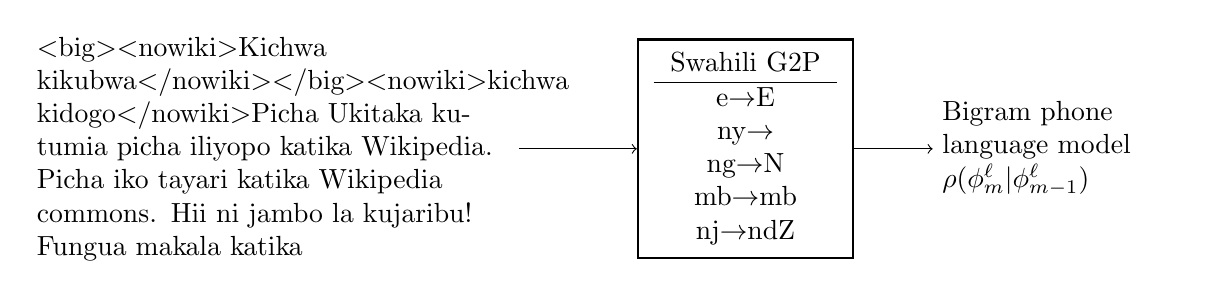
\begin{tikzpicture}[scale=\mytikzscale,every node/.style={transform shape}]
      \node[rectangle,text width=6cm](text) at (0,0) {$<$big$><$nowiki$>$Kichwa kikubwa$<$/nowiki$><$/big$><$nowiki$>$kichwa kidogo$<$/nowiki$>$Picha Ukitaka kutumia picha iliyopo katika Wikipedia.  Picha iko tayari katika Wikipedia commons. Hii ni jambo la kujaribu! Fungua makala katika};
      \node[rectangle,thick,draw=black,text width=2.5cm,text centered](dict) at (6,0) {\begin{tabular}{c}Swahili G2P\\\hline e$\rightarrow$\ipa{E}\\ny$\rightarrow$\ipa{\textltailn}\\ng$\rightarrow$\ipa{N}\\mb$\rightarrow$\ipa{mb}\\nj$\rightarrow$\ipa{ndZ}\end{tabular}} edge[<-](text);
      \node[rectangle,text width=3cm](pt) at (10,0) {Bigram phone language model $\rho(\phi_m^\ell |\phi_{m-1}^{\ell})$} edge[<-](dict);
    \end{tikzpicture}
  \end{center}
  \vspace*{-3mm}
  \caption{Bigram phone language model is trained using Wikipedia text
    (left) converted into phone strings using a character-based G2P
    (center).}
  \label{fig:wikitext}
\end{figure}

By assumption, phone bigram information is not available from speech:
we assume that there is no transcribed speech in the target language.
A reasonable proxy, however, can be constructed from text.
Fig.~\ref{fig:wikitext} shows text data downloaded from Wikipedia in
Swahili, and a segment of a character-based G2P for the Swahili
language.  {\color{blue} The G2P is constructed by looking up
  ``Swahili alphabet'' on wikipedia, downloading the resulting web
  page, and converting it by hand into an unweighted finite state
  transducer~\cite{Hasegawajohnson15}.}  By passing the former through
the latter, it is possible to generate synthetic phone sequences in
the target language.

Composing $PT\circ G$ is complicated by the presence of null
transitions in the PT.  A null transition in the PT matches a
non-event in the language model, for which normal FST notation has no
representation. In order to compose the PT with the language model,
therefore, it is necessary to introduce a special type of
``non-event'' symbol, here denoted ``\#2'', into the language model
(Fig.~\ref{fig:liu1}).  A language
model ``non-event'' is a transition that leaves any state, and returns
to the same state (a self-loop).  Such self-loops, labeled with the
special symbol ``\#2'' on both input and output language, are added to
every state in $G$ (Fig.~\ref{fig:liu1} (b)).
The probabilistic transcript, then, is
augmented with the special symbol ``\#2'' as the output-language symbol
for every null-input edge (input symbol is $\phi_m^\ell =\emptyset$).
\begin{figure}
\begin{center}
  \tikzstyle{pre}=[<-,shorten <=1pt,>=stealth',semithick,draw=black]
  \tikzstyle{post}=[->,shorten >=1pt,>=stealth',semithick,draw=black]
  \begin{tikzpicture}[
      scale=\mytikzscale,
      state/.style={circle,thick, draw=black, text=black, text width=0.25cm},
      compose/.style={circle,thick, draw=black, text=black, text width=0.1cm},
      every node/.style={transform shape}
    ]
    \node[state] (g0) at (-1.5,1) {};
    \node[state] (g1) at (1.5,1) {};
    \node[state] (g2) at (0,-1) {};
    \draw[post] (g0) -- (-1.75,1.5) -- (-1.5,1.75) -- (-1.25,1.5) -- (g0);
    \draw[post] (g0) -- (-2,0.75) -- (-2.25,1) -- (-2,1.25) -- (g0);
    \draw[post] (g1) -- (1.25,1.5) -- (1.5,1.75) -- (1.75,1.5) -- (g1);
    \draw[post] (g1) -- (2,1.25) -- (2.25,1) -- (2,0.75) -- (g1);
    \draw[post] (g2) -- (0.25,-1.5) -- (0,-1.75) -- (-0.25,-1.5) -- (g2);
    \draw[post] (g0) -- (g1);
    \draw[pre] (g0) -- (g2);
    \draw[pre] (g2) -- (g1);
    \draw[pre] (g0) -- (-1,1.5) -- (1,1.5) -- (g1);
    \draw[post] (g0) -- (-1.65,0.2) -- (-0.75,-1) -- (g2);
    \draw[post] (g2) -- (0.75,-1) -- (1.65,0.2) -- (g1);
    \node at (0,1.75) {a:a$/p(a|b)$};
    \node at (0,0.75) {b:b$/p(b|a)$};
    \node at (-3.25,1) {a:a$/p(a|a)$};
    \node at (3.25,1) {b:b$/p(b|b)$};
    \node at (-2,-0.5) {$\epsilon$:\#0$/\beta(a)$};
    \node at (-0.45,0.1) {a:a};
    \node at (2,-0.5) {b:b$/p(b)$};
    \node at (0.4,0.15) {$\epsilon$:\#0};
    \node at (-1.5,2) {\#2:\#2};
    \node at (1.5,2) {\#2:\#2};
    \node at (0,-2) {\#2:\#2};
    \node[text centered] at (0,-3) {(b) Language Model, $G$};
    %\node[compose] (c) at (4,0) {};
    \node[state] (pt0) at (-10,0) {};
    \node[state] (pt1) at (-8,0) {};
    \node[state] (pt2) at (-6,0) {};
    \node[compose] (pt2inner) at (-6,0) {};
    \draw[post] (pt0) -- (-9.5,0.5) -- (-8.5,0.5) -- (pt1);
    \draw[post] (pt0) -- (-9.5,-0.5) -- (-8.5,-0.5) -- (pt1);
    \draw[post] (pt1) -- (-7.5,0.5) -- (-6.5,0.5) -- (pt2);
    \draw[post] (pt1) -- (-7.5,-0.5) -- (-6.5,-0.5) -- (pt2);
    \node at (-9,0.75) {a:a$/0.8$};
    \node at (-9,-0.75) {$\emptyset$:\#2$/0.2$};
    \node at (-7,0.75) {b:b$/0.8$};
    \node at (-7,-0.75) {a:a$/0.2$};
    \node[text centered] at (-8,-3) {(a) Probabilistic Transcript, $PT$};
  \end{tikzpicture}
\end{center}
\vspace*{-2mm}
\caption{Deletion edges in the probabilistic transcript (edges with
  the special null-phone symbol, $\emptyset$), required special
  handling in order to use information from a phone language
  model.  As shown in (a), a new type of null symbol, ``\#2'', was invented
  to represent the output for every PT edge with an $\emptyset$ input.
  Such edges were only allowed to match with state
  self-loops, newly added to the language model (b) in order to
  consume such non-events in the transcript.  a,b: regular phone
  symbols, $\epsilon$: null-string, $p(b|a)$: bigram probability,
  $\beta(a)$: language model backoff.}
\label{fig:liu1}
\end{figure}


\subsection{Maximum {\em A Posteriori} Adaptation}
\label{sec:adaptation}

PT adaptation starts from a cross-lingual ASR,
and adapts its parameters to PTs in the target language.  The
Bayesian framework for maximum {\em a posteriori} (MAP) estimation
has been widely applied to GMM and HMM parameter estimation problems
such as speaker adaptation~\cite{gauvain1994maximum}.
Formally, for an unseen target language, denote its acoustic
observations $x = ( x_1^1, \ldots, x_{T}^L )$, and its acoustic model
parameter set as $\theta$, then the MAP parameters are defined as:
\begin{equation}
  \theta_{\mathrm{MAP}}  = \argmax_{\theta} \pi(\theta | x) 
= \argmax_{\theta} \pi( x | \theta ) \pi(\theta)
\label{eq:map}
\end{equation}
\noindent where $\pi(\theta)$ is the product of conjugate
prior distributions, centered at the parameters of a cross-lingual
baseline ASR.  In a GMM-HMM, the acoustic model 
is computed by choosing a Gaussian component, $G_t^\ell$, whose mixture
weight is $c_{jk}=\pi_{G_t^{\ell}|S_t^{\ell}}(k|j)$, and whose mean vector
and covariance matrix are $\mu_{jk}$ and $\Sigma_{jk}$.  Maximum
likelihood trains these parameters by computing
$\gamma^{\ell}_t(j,k)=\pi_{S_t^{\ell},G_t^{\ell}}(j,k|x^\ell,\theta)$,
then accumulating weighted average acoustic frames with weights given
by $\gamma_{t}^\ell(j,k)$. Segmental K-means quantizes
$\pi_{S_t^\ell}(j|x^\ell,\theta)\rightarrow\left\{0,1\right\}$ using forced
alignment, then proceeds identically.  MAP adaptation assigns, to each
parameter, a conjugate prior $\pi(\theta)$ with mode equal to
$\bar\theta$ (the parameters of the cross-lingual baseline), and with a
confidence hyperparameter $\tau_\theta$, resulting in re-estimation
formulae that are linearly interpolated between the baseline
parameters $\bar\theta$ and the statistics of the adaptation data, for
example:
\begin{equation}
c_{jk}'=\frac{\tau_c\bar{c}_{jk}+\sum_{\ell,t}\gamma_{t}^\ell(j,k)}
{\sum_{n}\left(\tau_c\bar{c}_{jn}+
  \sum_{\ell,t}\gamma_{t}^\ell(j,n)\right)}
\end{equation}



\subsection{Neural Networks}

The NN acoustic model is $\pi_{X_t^{\ell}|S_t^\ell}(v|j,\theta)\propto y_t^\ell(j)$,
\begin{equation}
y_t^\ell(j)=\frac{1}{c_j}\frac{\exp\left(w_j^Th_t(v,w_{vh})\right)}
{\sum_k \exp\left(w_k^Th_t(v,w_{vh})\right)}
\end{equation}
whose parameters $\theta=\left\{c_j,w_j,w_{vh}\right\}$ include the
senone priors $c_j$, the softmax weight vectors $w_j$, and the
parameters defining the hidden nodes $h_t(v,w_{vh})$.  NNs are
trained by using a GMM-HMM to compute an initial senone posterior,
$\pi_{S_t^{\ell}}(j|x^\ell,\theta)$, then minimizing the cross-entropy
between the estimated senone posterior and the neural network output
$y_{t}^\ell(j)$,
using gradient descent in the direction
\begin{equation}
  -\nabla_\theta H(S^\ell\Vert Y^\ell)=
  \sum_{t=1}^T\sum_j\frac{\pi_{S_t^{\ell}}(j|x^\ell,\theta)}{y_t^\ell(j)}
  \nabla_\theta y_t^\ell(j)
  \label{eq:dnn_dt}
\end{equation}
Preliminary experiments showed that forced alignment improves the
accuracy of NNs trained from probabilistic transcripts: the best path
through the PT, and the best alignment of the resulting senones to the
waveform, were both computed using forced alignment.  The resulting
best senone string was used to train a NN using Eq.~(\ref{eq:dnn_dt}).



% Section 5: Audio Data and Mismatched Crowdsourcing
%\subsection{Data}
\section{Audio Data and Mismatched Crowdsourcing}
\label{sec:data}

Speech data were extracted from publicly available podcasts~\cite{SBS}
hosted in 68 different languages.  In order to generate test corpora
(in which it is possible to measure phone error rate), advertisements
were posted at the University of Illinois seeking native speakers
willing to transcribe speech in any of these 68 languages.  Of the ten
transcribers who responded, six people were each able to complete one
hour of speech transcription (the other four dropped out).  One
additional language was transcribed by workers recruited at $I^2R$ in
Singapore, yielding a total of seven languages with native
transcripts suitable for testing an ASR: Arabic (arb), Cantonese
(yue), Dutch (nld), Hungarian (hun), Mandarin (cmn), Swahili (swh) and
Urdu (urd).
It is desirable to test the ideas in this paper with corpora larger
than one hour per language, but larger corpora involve problems
orthogonal to the purposes of this paper, e.g., the Babel corpora
contain telephone speech, and therefore contain far more acoustic
background noise than the podcast corpora used in this paper.

The podcasts contain utterances interspersed with segments of music
and English. A GMM-based language identification system was
developed in order to isolate
regions that correspond mostly to the target language, which
were then split into 5-second
segments to enable easy labeling by the native transcribers.
Native transcribers were asked to omit any 5-second clips that
contained significant music, noise, English, or speech from multiple
speakers. Resulting transcripts covered 45 minutes of speech in Urdu
and 1 hour of speech in the remaining six languages. The orthographic
transcripts for these clips were then converted into phonemic
transcripts using language-specific dictionaries and G2P mappings.
In order to make it possible to transfer ASR from
training languages (which have native transcripts) to a test
language (that has no native transcripts), the phone set must be
standardized across all languages; for this purpose, the phone set
was based on the international phonetic alphabet
(IPA;~\cite{ipa1993}).  Similarly, in order to transfer ASR from
training languages to a test language, the training transcriptions
must be converted to phonemes using a grapheme-to-phoneme transducer
(G2P).  G2Ps were therefore assumed to be available in all training
languages, but not in the test language.  Since these G2Ps are only
used for training and not test languages, five of them (Arabic,
Dutch, Hungarian, Cantonese and Mandarin) were trained using lexical
resources, and only two (Urdu and Swahili) were constructed using
the zero-resource knowledge-based method described in
Sec.~\ref{sec:trainwithlm}.  English words in each transcript are
identified and converted to phones with an English G2P trained using
CMUdict~\cite{Lenzo1995}, then other words are converted into phonetic
transcripts using language-dependent dictionaries and G2Ps.
The Arabic dictionary is from the Qatari Arabic Corpus~\cite{Elmahdy14},
the Dutch dictionary is from CELEX v2~\cite{Baayen96},
the Hungarian dictionary was provided by BUT~\cite{Grezl14},
the Cantonese dictionary is from $I^2R$,
and the Mandarin dictionary is from CALLHOME~\cite{LDC96}.
For
each language, we chose a random 40/10/10 minutes split into training,
development and evaluation sets.

%\subsection{Mismatched Crowdsourcing}
\label{sec:methodsmc}

Mismatched transcripts were collected from crowd workers (Turkers)
on Amazon Mechanical Turk.
%for all the data listed in
%Table~\ref{tab:data}.  The crowdsourcing task setup is described
%in~\cite{JHJ15b}.
Each 5-sec speech segment was further split into 4
non-overlapping segments to make the non-native listening task
easier. The crowdsourcing task was set up as described
in~\cite{JHJ15b}; briefly, the segments were played to Turkers,
who transcribed what they heard (typically in the form of nonsense
syllables) using English orthography. Each segment was
transcribed by 10 distinct Turkers. More than 2500 Turkers
participated in these tasks, with roughly 30\% of them claiming to
know only English (Spanish, French, German, Japanese, Chinese were
some of the other languages listed by the Turkers).


%\subsection{Mismatched Crowdsourcing}
\label{s6:mc}

%\begin{figure}
%  \centerline{\includegraphics[width=0.7\columnwidth]{../figs/lm_results.pdf}}
%  \vspace*{-0.7cm}
%  \caption{LPER of the 1-best path: a measure of the quality of
%    probabilistic transcripts acquired from mismatched
%    crowdsourcing.  Native transcripts were available in six
%    languages: Swahili (swh), Dutch (nld), Mandarin (cmn), Urdu (urd),
%    Arabic (arb), and Hungarian (hun).  Probabilistic transcripts
%    were decoded using three different methods per language: using a
%    universal phone set (leftmost bar in each language), using a
%    phone set specific to the target language (middle bar in each
%    language), and using a phonotactic language model derived from
%    Wikipedia texts (rightmost bar in each language).}
%  \label{fig:pt_decode_per}
%\end{figure}

The quality of a probabilistic transcript derived from mismatched
crowdsourcing is significantly improved by using a phone language
model during the decoding process ($\rho(\phi)$ in Eq.~(\ref{eq:PT})).
%A crude measure of the quality of the PTs is given by the label phone error
%rate (LPER), which measures the difference
%between $\phi^* = \argmax_{\phi} \rho(\phi|T)$ and a native transcript.
Phone
language models for each target language were computed from Wikipedia
texts using the methods described in Sec.~\ref{sec:trainwithlm}.
Label phone error rate
(LPER) of the 1-best path through the resulting PTs are shown in
Table~\ref{fig:pt_decode_per}, computed with reference to a native
transcript in each language.  As shown, the use of a phone
language model, derived from Wikipedia text, reduces LPER by about 10\%
absolute, in each language.

\begin{table}
\centerline{\begin{tabular}{|c||c|c|c|c|c|c|}\hline
    Method & nld & cmn & urd & arb & hun &swh \\\hline
    Universal set & 87.4 & 88.86 & 97.95 & 79.04 & 92.87 & 88.56 \\
    Target set & 78.12 & 87.4 & 87.81 & 66.39 & 84.78 & 59.83 \\
    Phone bigram & 70.43 & 70.88 & 64.67 & 65.29 & 63.98 & 50.45 \\\hline
\end{tabular}}
\vspace*{1mm}
\caption{Label phone error rate (LPER) of probabilistic transcripts
  for universal phone set, target-language phone set, text-based
  phone bigram.}
\label{fig:pt_decode_per}
\end{table}

%\begin{table}[t]
%\centering
%\begin{tabular}{|c||c|c|c|c|c|c|c|}
%  \hline
%  & \multicolumn{7}{|c|}{Language (ISO 639-3 Code)}\\ \hline
%& arb & yue & nld & hun & cmn & swh & urd \\ \hline\hline
%Dev set (1-best PER) & 65.8 & 66.4 & 68.9 & 63.7 & 70.9 & 47.6 & 67.2 \\
%Eval set (1-best PER) & 66.2 & 67.8 & 70.9 & 63.5 & 69.6 & 50.3 & 70.5 \\\hlineswh	88.05	59.78	48.08

%\end{tabular}
%\caption{Error rates (PER) of probabilistic transcripts computed from
%  mismatched crowdsourcing (non-native human listener): Phone error
%  rate (PER) of the 1-best path through the probabilistic
%  transcript, $\phi^*=\argmax\rho(\phi|T)$, development and
%  evaluation sets.}
%\label{tab:LPER}
%\end{table}

%Table~\ref{tab:LPER} lists LPERs on the development and evaluation
%sets, for all seven languages.
LPER of the 1-best path does not
accurately reflect the extent of information in the PTs that can be
leveraged during ASR adaptation.  Consider, for example, the four
Urdu phones~\ipa{[p,p\textsuperscript{h},b,b\textsuperscript{H}]}.  An attentive
English-speaking transcriber must choose between the two letters
$<$p,b$>$ in order to represent any of these four phones.  The
misperception G2P therefore maps the letters $<$p,b$>$ into a
distribution over the phones~\ipa{[p,p\textsuperscript{h},b,b\textsuperscript{H}]}.
There is no reason to expect that the maximizer of
$\rho(\phi|\lambda)$ is correct, but there is good reason to expect
the correct answer to be a member of a short $N$-best list ($N\le 4$
phones/grapheme).  A fuller picture is therefore obtained by
{\color{blue} pruning the PT to
a small number of paths, then searching for the most correct path
in the pruned PT.  One useful metric is entropy per segment, defined
as $H^{\ell}(\Phi)=-\frac{1}{M}\sum_{m=1}^M\sum_{u} \log_2\rho_{\Phi_m^\ell}(u)$,
e.g., a PT in which every segment has two equally probable options 
would measure $H^\ell(\Phi)=1$.}
Fig.~\ref{fig:listPER}
shows the trend of LPER (for three languages) obtained by pruning
the PT at several different levels of $H^{\ell}(\Phi)$.
LPER rates drop significantly across all languages within 1
bit of entropy per phone, illustrating the extent of information
captured by the PTs.

\begin{figure}[t!]
  %\centerline{\includegraphics[width=0.7\columnwidth]{../figs/ptperfigure.pdf}}
  \input{../figs/listper.tex}
  \vspace*{-0.5cm}
  \caption{LPER plotted against entropy rate estimates of phone sequences in three different languages.}
\label{fig:listPER}
\end{figure}



% Section 6: EEG methods and results
\subsection{EEG Recording and Analysis}
\label{sec:methods_eeg}

To compute distinctive feature weights for the misperception
transducer shown in Eqs.~(\ref{eq:dfdist}) and~(\ref{eq:eegdist}),
cortical activity in response to non-native phones was recorded by
an EEG. Signals were acquired using a BrainVision actiCHamp 
system with 64 channels and 1000 Hz sampling frequency.
All procedures were approved by the University of Washington Institutional
Review Board.

%% This next section, including tab:m2o, seems like more detail than
%% is necessary; the explanation above as to **why** we chose Hindi and
%% Dutch (combined with tab:eegphones) seems sufficient here, without
%% going into the extra details of **how** we settled on those two.
% MH: I feel like it's useful to include at least some of this information.
% I could imagine different ways to define the ``number of many-to-one
% mappings,'' other than the metric listed in eq:m2o.
% Somebody someday might come back and test different versions of this
% metric to see which one is most useful, for some definition of ``useful.''
%% DM: point conceded, though I still think the table is overkill.
Auditory stimuli were consonant-vowel
(CV) syllables representing consonants of three languages: English,
Dutch and Hindi. The inclusion of only two non-English languages 
was dictated by the relatively high number of
repetitions needed for good signal-to-noise ratio from averaged
EEG recordings. The choice of Dutch and Hindi was made based on language
phonological similarity, defined as the number of many-to-one mappings
($N_{M2O}$) between the English phoneme inventory
and the non-English phoneme inventory.
Many-to-one mappings are expected to pose a problem for the 
non-native transcription task being modeled by the misperception 
transducer, so to test the contribution of EEG we chose languages that 
differed greatly in this property. 
Using distinctive feature representations of the phonemes in each
inventory from the PHOIBLE database~\cite{phoible}, a many-to-one 
mapping was defined by finding, for each
non-English phoneme $\phi$, the English phoneme $\psi^*(\phi)$ to which
it is most similar.
%\begin{equation}
%  \psi^*(\phi) = \argmin \sum_k \delta\left(f_k(\psi)\ne f_k(\phi)\right)
%\end{equation}
The number of many-to-one collisions is then defined as
\begin{equation}
  N_{M2O}=\frac{1}{|\Omega_\Psi|}\sum_{\phi_1\ne\phi_2}
  \left[\psi^*(\phi_1)=\psi^*(\phi_2)\right]
\label{eq:m2o}
\end{equation}
where $|\Omega_\Psi|$ is the size of the English phoneme inventory,
and $\left[\cdot\right]$ is the unit indicator function.
The frequency of many-to-one mappings is listed in
Table~\ref{tab:m2o} for several languages.
Hindi was chosen for having a large number of
many-to-one mappings with English, while Dutch has relatively few. 
%% rest of this paragraph could probably be cut if necessary
Note that, although Hindi podcasts were not included in the training
data described in Section~\ref{sec:data}, colloquial spoken Hindi and
Urdu are extremely similar phonologically~\cite{Kachru90}, and
considering that the auditory stimuli for the EEG portion of this
experiment are simple CV syllables, it is reasonable to consider Hindi
and Urdu as equivalent for the purpose of computing feature weights for
the misperception transducer.

\begin{table}
  \centerline{\begin{tabular}{|lr|lr|lr|}\hline
    Language & $N_{M2O}$ &
    Language & $N_{M2O}$ &
    Language & $N_{M2O}$ \\ \hline
    spa & 0.862 & yue & 1.280 & cmn & 1.531 \\
    por & 1.152 & jpn & 1.333 & amh & 1.844 \\
    nld & 1.182 & vie & 1.393 & hun & 1.857 \\
    deu & 1.258 & kor & 1.429 & hin & 2.848 \\\hline
  \end{tabular}}
  \vspace*{1mm}
  \caption{Frequency of many-to-one mappings $N_{M2O}$
    between other languages' phoneme inventories and the inventory of
    English. Languages are represented by their ISO 639-3 codes.}
  \label{tab:m2o}
\end{table}

To construct the auditory stimuli, two vowels and several consonants
were selected from the phoneme inventory of each language (18 consonants
for English, 17 for Dutch, and 19 for Hindi). Consonants were chosen
to emphasize differences in the many-to-one relationships
between English-Dutch and English-Hindi, while maintaining roughly equal 
numbers of consonants for each language. The consonants chosen for each 
language are given in Table~\ref{tab:eegphones}; the vowels chosen were 
the same for all three languages (/a/ and /e/).

\begin{table}
  \centering
  \setlength{\tabcolsep}{0.3em}
  \setlength\extrarowheight{2pt}
  \begin{tabular}{|l||cc|cccc|cc|c|c|c|c|c|c|c|}\hline
     & \multicolumn{15}{c|}{Consonants used in the EEG experiment}\\ \hline\hline
    eng & \multicolumn{2}{c|}{p} & \multicolumn{4}{c|}{t} & \multicolumn{2}{c|}{k} & \textipa{tS} & v & \textipa{D} & z & m & \multicolumn{2}{c|}{n} \\\hline
    nld &  \multicolumn{2}{c|}{p} & \multicolumn{4}{c|}{t} & \multicolumn{2}{c|}{\textipa{G}} & & v & & z & m & \multicolumn{2}{c|}{n} \\\hline
    hin &  p & b & \textipa{\|[t} & \textipa{\|[d} & \textipa{\:t} & \textipa{\:d} & k & \textipa{g} & & \textipa{V} & & & m & \textipa{\|[n} & \textipa{\:n} \\\hline\hline
    eng & \multicolumn{2}{c|}{\textipa{p\super h}} & \multicolumn{4}{c|}{\textipa{t\super h}} & \multicolumn{2}{c|}{\textipa{k\super h}} & \textipa{tS\super h} & f & \textipa{T} & \textipa{S} & l & \textipa{\*r} & \\\hline
    nld & \multicolumn{2}{c|}{\textipa{p\super h}} & \multicolumn{4}{c|}{\textipa{t\super h}} & \multicolumn{2}{c|}{\textipa{k\super h}} & \textipa{tS\super h} & f & & \textipa{S} & l & \textipa{\;R} & j \\\hline
    hin & \multicolumn{2}{c|}{\ipa{b\super H}} & \textipa{\|[t\super h} & \textipa{\:t\super h} & \textipa{\textsubbridge{d}\super H} & \textipa{\:d\super H} & \textipa{k\super h} & \textipa{g\super H} & & & & & &&\\\hline
  \end{tabular}
  \vspace*{1mm}
  \caption{Consonant phones used in the EEG experiment represented using
  IPA. Vertical alignment of cells suggests many-to-one mappings
  expected based on distinctive feature values.}
  \label{tab:eegphones}
\end{table}

Two native speakers of each language (one male and one female) were
recorded (44100 Hz sampling frequency, 16 bit depth) speaking multiple 
repetitions of the set of CV syllables for
their language. Three tokens of each unique syllable were excised from
the raw recordings, downsampled to 24414 Hz (for compatibility with the
presentation hardware, Tucker Davis Technologies RP2.1), and RMS normalized.
Recorded syllables had an average duration of 400~ms, and were presented
via headphones to one monolingual American English listener.
The stimuli were presented in 9 blocks of 15 minutes per block, for a
total of 135 minutes.  Syllables were presented in random order with an
inter-stimulus interval of 350~ms. Twenty-one repetitions of each syllable
were presented, for a grand total of 9072 syllable presentations.

%% TODO: get number of ms where epoch started (MM to email GDL)
EEG recordings were divided into 500 ms epochs.
The epoched data were coded with a subset of distinctive features
that minimally defined the phoneme contrasts of the English consonants.
Where more than one choice of features was sufficient to define those
contrasts, preference was given to features that reflect differences
in temporal as opposed to spectral features of the consonants, due to
the high fidelity of EEG at reflecting temporal envelope properties of 
speech~\cite{Liberto15}. The final set of features chosen was:
continuant, sonorant, delayed release, voicing, aspiration, labial,
coronal, and dorsal.
% In other words, differences in the temporal amplitude envelope of
% consonants have a better chance of being recoverable after being
% filtered through a human auditory system and cortex than do differences
% that are purely spectral in nature; to the extent that spectral
% information in speech is preserved in an EEG signal, it will have been
% transformed to be spatially coded across populations of neurons.


\label{ssec:eeg}

\newcommand{\specialcell}[2][c]{%
  \begin{tabular}[#1]{@{}c@{}}#2\end{tabular}}

Epoched and feature-coded EEG data {\em for the English syllables
only} were used to train a support vector machine classifier for each
distinctive feature.  The classifiers were then used (without
re-training) to classify the EEG responses to the Dutch and Hindi
syllables.  Fig.~\ref{fig:eeg_svm_eers} shows equal error rates of
these classifiers when applied to the three languages. 
EER of the classifier when applied to English phones is comparable to
those reported in~\cite{Liberto15}, the only prior work to attempt a
recognition of speech phonemes from EEG of the listener.

\begin{figure}
  \centerline{\includegraphics[width=\columnwidth]{../figs/eer-barplot/eer-barplot.pdf}}
  \vspace*{-0.3cm}
  \caption{Classifiers were trained to observe EEG signals, and to
    classify the distinctive features of the phone being heard.  Equal
    error rates are shown for English (the language used in training;
    train and test data did not overlap), Dutch, and Hindi.  Dashed
    line shows chance=50\%.}
  \label{fig:eeg_svm_eers}
\end{figure}

Eq.~(\ref{eq:dfdist}) defines a log-linear model of $\rho(\psi|\phi)$,
the probability that a non-English phoneme $\phi$ will be perceived as
English phoneme $\psi$.  Denote by $\rho_U(\psi|\phi)$ the model of
Eq.~(\ref{eq:dfdist}) with uniform binary weights for all distinctive
features. Denote by $\rho_{EEG}(\psi|\phi)$ the same model, but with
weights $w_k$ derived from EEG measurements (Eq.~(\ref{eq:eegdist})).
Fig.~\ref{fig:eeg_confusions} shows these two confusion matrices:
$\rho_U(\psi|\phi)$ on the left, $\rho_{EEG}(\psi|\phi)$ on the
right. The entropy of the binary weighting, $\rho_U(\psi|\phi)$, is
too low: when a Dutch phoneme $\phi$ has a nearest-neighbor
$\psi^*(\phi)$ in English, then few other phonemes are considered to
be possible confusions.  $\rho_{EEG}(\psi|\phi)$ has a very different
problem: since distinctive feature classifiers have been trained for
only a small set of distinctive features, there are large groups of
phonemes whose confusion probabilities can not be distinguished
(giving the figure its block-matrix structure).  The faults of both
models can be ameliorated by averaging them in some way, e.g., by
computing the linear interpolation
$\rho_I(\psi|\phi)=(1-\alpha)\rho_U(\psi|\phi)+\alpha\rho_{EEG}(\psi|\phi)$
for some constant $0\le\alpha\le 1$.

\begin{figure}
  \centerline{
    \includegraphics[width=\columnwidth]{../figs/confusion-matrix/confusion-matrices.pdf}
  }
    \vspace*{-0.3cm}
  \caption{Phone confusion probabilities between English and Dutch
    phones using models in which the negative log
    probability is proportional to unweighted or weighted
    distance between the corresponding
    distinctive feature vectors.  Left: unweighted.
    Right: feature weights equal negative log confusion
    probability of EEG signal classifiers.}
  \label{fig:eeg_confusions}
\end{figure}

In order to evaluate the effectiveness of the EEG-induced
misperception transducer we looked at the LPER of mismatched
crowdsourcing for Dutch when performed using 1)~a multilingual
misperception model $\rho(\lambda|\phi)$ (the machine translation
model described in Sec.~\ref{sec:MC}), 2)~feature-based misperception
transducer computed using binary weighting, $\rho_U(\psi|\phi)$, or 3)
EEG-induced transducer combined with the feature-based transducer,
$\rho_I(\psi|\phi)$.  Both method (2) and method (3)
required the use of a G2P in order to compute $\rho(\lambda|\psi)$:
the Dutch G2P was estimated using the CELEX database, while the Hindi
G2P was estimated using the zero-resource knowledge-based method
described in Sec.~\ref{sec:trainwithlm}.  The constant $\alpha=0.29$ was
chosen as the average of the values selected by all folds in a
leave-one-out cross-validation.  LPER of the multilingual model was
70.43\% (as shown in Table~\ref{fig:pt_decode_per}), of
the feature-based model, 69.44\%, and of the EEG-interpolated model,
68.61\%.





% Section 7: ASR methods and results
%%%%%%%%%%%%%%%%%%%%%%%%%%%%%%%%%%%%%%%%%%%%%%%%
%\section{Experimental Methods}
\section{Automatic Speech Recognition}
\label{sec:methods}

ASR was trained in four target languages in topline,
baseline, and experimental conditions. Training methods are detailed
in Sec.~\ref{sec:mlbaseline}.  Results are desribed in
Sec.~\ref{ssec:asr}.


%\subsection{Cross-Lingual Baselines}
\subsection{ASR Methods}
\label{sec:mlbaseline}

Automatic speech recognition (ASR) systems were trained
in four languages (hun=Hungarian, cmn=Mandarin, swa=Swahili,
yue=Cantonese), using three different types of transcription.
First, a topline {\sc monolingual} system was trained in each
language using speech transcribed by a native speaker of that
language.  Second, a baseline {\sc CL} (cross-lingual) system was
trained using data from other languages, and tested in the target
language.  Third, the experimental {\sc PT-adapt} system was created
by adapting the cross-lingual system to probabilistic transcriptions
in the target language.  The {\sc monolingal} topline system is
trained using native transcripts, and converted to the phone set of
the test language using the G2Ps described in Sec.~\ref{sec:data}.
These resoures were not available to the {\sc CL} or {\sc PT-adapt}
systems, which were not permitted to use any natively transcribed
training data in the test language.

Audio data, native transcripts, and probabilistic
transcripts are as described in Sec.~\ref{sec:data}.  The {\sc
  monolingual} topline system was trained using 40 minutes of
training data, then stream weights and insertion penalties were
calculated using 10 minutes of development test data.  Monolingual
systems were trained using a maximum likelihood (ML) criterion using
the 40 minute in-language training set: GMM parameters were
initialized using a monophone system trained on the same 40 minutes,
NN parameters were initialized using a restricted Boltzmann machine
trained on five hours of unlabeled audio in the same language.  The
{\sc CL} baseline systems were each trained using 40 minutes of
training data in languages other than the test language.  CL systems
were trained using ML, maximum mutual information (MMI), minimum
phone error rate (MPE), and state-based minimum Bayes risk
(sMBR,~\cite{Gibson06}) training criteria.  The {\sc PT-adapt}
system was initialized using the CL system (ML training), then
adapted to the target language using PTs based on mismatched
crowdsourcing (these transcripts are described in detail in
Sec.~\ref{sec:data}).  Probabilistic transcripts based on EEG were
not used to adapt ASR, because it is not yet possible to use EEG to
generate probabilistic transcripts on a scale sufficient for ASR
adaptation.
    
All systems were trained using the Kaldi~\cite{Kaldi2011}
toolkit. Acoustic features consisted of MFCC (13
features), stacked $\pm 3$ frames ($13\times 7=91$ features),
reduced to 40 dimensions using LDA followed by fMLLR.  GMM-HMM
systems directly observed this 40-dimensional vector; NN-HMM systems
computed fMLLR+d+dd stacked $\pm 5$ frames ($40\times 3\times
11=1320$ features/frame).  All systems used tied triphone acoustic
models, based on a decision tree with 1200 leaves.  Each GMM-HMM
used a library of 8000 Gaussians, shared among the 1200 leaves.
Each NN-HMM used six hidden layers with logistic nonlinearities, and
with 1024 nodes per hidden layer, followed by a softmax output layer
with 1200 nodes.
  



%\subsection{MAP Adaptation to Probabilistic Transcripts}
\label{sec:ptadapt}

The {\sc PT-adapt} system was
adapted using MAP adaptation (Sec.~\ref{sec:adaptation})
co mputed over weighted finite state transducers in 
Kaldi~\cite{Kaldi2011}. In order to efficiently carry out the required
operations on the cascade $H\circ C\circ PT\circ G$,
the cascade for $PT$ includes an
additional wFST restricting the number of consecutive deletions of
phones and insertions of letters (to a maximum of 3).
MAP adaptation for
the acoustic model was carried out for a number of iterations (12 for
yue \& cmn, 14 for hun \& swh, with a re-alignment stage in iteration
10).

%\subsection{Cross-Lingual Baseline}
\subsection{ASR Results}
\label{s6:mlbaseline}

Tables~\ref{tab:ptresult} and~\ref{tab:dnnresult} present phone error
rates (PERs) for four different languages.  {\color{blue} The first
  column shows the phone error rate (PER) of monolingual topline
  systems: evaluation test results are followed by development test
  results in parentheses.}  The column titled {\sc CL} lists
cross-lingual baseline error rates.  The column labeled {\sc ST} lists
the PERs of self-trained ASR systems.  The column headed {\sc
  PT-adapt} in Table~\ref{tab:ptresult} lists PERs from {\sc CL} ASR
systems that have been adapted to PTs {\color{blue} derived from
  mismatched crowdsourcing. Phone error rates are reported instead of
  word error rates because, in order to compute a word error rate, it
  is necessary to have either native transcriptions in the target
  language (thereby permitting the training of a grapheme-based
  recognizer) or a pronunciation lexicon in the target language.
  These resources are used by the monolingual topline, but not by any
  of the baseline or experimental systems.}

%The first four columns of
%Table~\ref{tab:ptresult}  

%compare a monolingual ASR with phone language model based on
%monolingual transcripts, a 
%cross-lingual ASR using universal phone set and
%phone language model, and a cross-lingual ASR using a
%phone language model based on language-dependent Wikipedia texts.

%Without a language specific phone set
%and phone language model, it is hard for a cross-lingual system to
%generalize to an unseen language.  This is true even if the system has
%seen closely related languages such as Mandarin when tested on
%Cantonese.  
%
%\begin{table*}
%\begin{center}
%\begin{tabular}{|c|c|c|cccc|}
%\hline
%data & acoustic & language & yue & hun & cmn & swh \\
% & model & model &  & & & \\
%\hline
%cross-lingual & GMM & cross-lingual & 79.64 (79.83) & 77.13 (77.85) & 83.28 (82.12) & 82.99 (81.86) \\
%cross-lingual & NN & cross-lingual & 78.62 (77.58) & 75.98 (76.44) & 81.86 (80.47) & 82.30 (81.18) \\
%cross-lingual & GMM & text & 68.40 (68.35) & 68.62 (66.90) & 71.30 (68.66) & 63.04 (64.73) \\
%cross-lingual & NN & text & 66.54 (65.28) & 66.08 (66.58) & 65.77 (64.80) & 64.75 (65.04) \\
%\hline
%monolingual & GMM & transcript & 32.77 (34.61) & 39.58 (39.77) & 32.21 (26.92) & 35.33 (46.51) \\
%monolingual & NN & transcript & 27.67 (28.88) & 35.87 (36.58) & 27.80 (23.96) & 34.98 (41.47) \\
%\hline
%\end{tabular}
%\vspace*{1mm}
%\caption{\label{tab:results} PERs of unadapted cross-lingual
%  and monolingual ASR on
%  the evaluation sets (development sets are in parentheses).
%  Text-based language models are
%  trained using Wikipedia.
%  Transcript-based
%  language models are based on
%  native transcripts of the training data.}
%\end{center}
%\end{table*}

The monolingual ASR is trained using only 40 minutes of audio and
transcript data per language, but performs reasonably well (31.58\%
average PER, NN-HMM).  The cross-lingual ASRs, however, perform poorly.
%From the comparison of different baseline systems, we can reach the
%following conclusions.  First, even with only 40 minutes of
%training data, a NN is able to outperform a GMM.  Second,
%however, the standard speech pipeline performs poorly on unseen languages.
Using a text-based phone bigram (denoted {\sc TEXT}) gives significant
improvement over the cross-language phone bigram (denoted {\sc CL}),
but significantly underperforms a system that has seen the test
language during training.  This is true even if the system has seen
closely related languages during training: the Cantonese cross-lingual
system has seen Mandarin during training, and the Mandarin system has
seen Cantonese during training, but neither system is able to
generalize well from its six training languages to its test language.
{\color{blue} Three different types of discriminative training were
  tested.  MMI performs consistently worse than MPE and sMBR, and is
  therefore not listed in Table~\ref{tab:ptresult}.  Averaged across
  all languages and systems shown in Table~\ref{tab:ptresult}, the
  development-test PERs of ML, MPE, and sMBR training are 73.43\%,
  73.04\%, and 72.98\% respectively; differences are not statistically
  significant, therefore only the ML system was tested on evaluation
  test data.}


%\input{s6_results.tex}
%\subsection{ASR Trained Using Probabilistic Transcripts}
\label{ssec:asr}

\setlength{\tabcolsep}{0.1cm}
\begin{table*}[t]
\centerline{\begin{tabular}{| c || c | c c c | c c c | c c c |}\hline
    AM& Monolingual&\multicolumn{6}{c|}{Cross-Lingual ({\sc CL})}
    &\multicolumn{3}{c|}{CL + PT adaptation ({\sc PT-adapt})}
    \\\hline
    LM & Transcript& \multicolumn{3}{c|}{CL}&
    \multicolumn{3}{c|}{Text} &
    \multicolumn{3}{c|}{Text}
    \\\hline
    Training & ML & ML & MPE & sMBR & ML & MPE & sMBR & ML & MPE & sMBR
    \\\hline\hline
    yue & 32.77 (34.61)
    & 79.64 (79.83) & (79.49) & (79.48) 
    & 68.40 (68.35) & (68.02) & (66.94) 
    &  57.20** (56.57)
    &  56.33** (55.70)
    & \textbf{55.97}** (55.51)
    \\
    hun & 39.58 (39.77)
    & 77.13 (77.85) & (78.67) & (78.89)
    & 68.62 (66.90) & (67.09) & (67.41)
    & \textbf{56.98}** (57.26)
    & 57.05** (56.95)
    & 57.05** (57.18)
    \\
    cmn & 32.21 (26.92)
    & 83.28 (82.12) & (81.60) & (81.76)
    & 71.30 (68.66) & (66.35) & (66.02)
    & 58.21** (57.85)
    & 55.17** (54.49)
    & \textbf{55.07}** (54.94)
    \\
    swh & 35.33 (46.51)
    & 82.99 (81.86) & (81.80) & (82.32)
    & 63.04 (64.73) & (63.48) & (62.99)
    & 44.31** (48.88)
    & \textbf{42.80}** (46.77)
    & 43.61** (46.55)
    \\\hline
\end{tabular}}
\vspace*{1mm}
\caption{\label{tab:ptresult} Phone error rate of GMM-HMMs: evaluation test (development test).  AM=Acoustic Model, LM=Language Model, ML=Maximum Likelihood, sMBR=State-based Minimum Bayes Risk.  MAPSSWE w/respect to CL: ** denotes $p<0.001$.}
\end{table*}

\setlength{\tabcolsep}{0.1cm}
\begin{table*}[t]
\centerline{\begin{tabular}{| c || c | c c c | c c c | c | c |}\hline
    AM& Monolingual&\multicolumn{6}{c|}{Cross-Lingual ({\sc CL})}&Self-training
    ({\sc ST})    &CL + PT adaptation ({\sc PT-adapt})
    \\\hline
    LM & Transcript& \multicolumn{3}{c|}{CL}&
    \multicolumn{3}{c|}{Text} & Text & Text
    \\
    Training & ML & ML & MPE & sMBR & ML & MPE & sMBR & ML & ML 
    \\\hline\hline
    yue & 27.67 (28.88)
    & 78.62 (77.58) & (77.86) & (77.92) 
    & 66.59 (65.28) & (65.76) & (65.76)
    & 63.79ns (62.46)
    & \textbf{53.64}** (53.80)
    \\
    hun & 35.87 (36.58)
    & 75.98 (76.44) & (77.56) & (77.61)
    & 66.43 (66.58) & (65.52) & (65.67)
    & 63.53ns (63.50)
    &   \textbf{56.70}** (58.45)
    \\
    cmn & 27.80 (23.96)
    & 81.86 (80.47) & (81.02) & (80.93)
    & 65.77 (64.80) & (63.90) & (63.82)
    & 64.90ns (64.00)
    &   \textbf{54.07}** (53.13)
    \\
    swh & 34.98 (41.47)
    & 82.30 (81.18) & (81.30) & (81.24)
    & 65.30 (65.04) & (63.78) & (63.99)
    & 58.76* (59.81)
    &   \textbf{44.73}** (48.60)
    \\\hline
\end{tabular}}
\vspace*{1mm}
\caption{\label{tab:dnnresult} PER of NN-HMMs: evaluation test (development test).  ML=Maximum Likelihood, MPE=minimum phone error, sMBR=state-level Minimum Bayes Risk.  MAPSSWE w/respect to CL AM w/ text-based LM: * means $p<0.002$, ns=not significant. ** denotes a score lower than both CL and ST at $p<0.001$.}
\end{table*}

%This section demonstrates that PT adaptation improves the
%generalization capability of cross-lingual ASR to an unseen target
%language.  Adaptation to ASR-derived PTs (self-training) significantly
%reduces PER, as has been previously
%reported~\cite{vesely2013-semi}. PTs derived from human mismatched
%crowdsourcing provide significant further PER reduction.

{\color{blue} Evaluation test PER of each experimental system (columns
{\sc ST} and {\sc PT-adapt}, 20 systems) was compared to evaluation test PER of
the corresponding {\sc CL} system ({\sc ML} training, {\sc Text} LM)}
%Differences between the evaluation set PERs of {\sc ST} and {\sc CL}
%systems were tested for statistical significance
using the MAPSSWE test of the {\tt sc\_stats} tool~\cite{Pallet90}.
{\color{blue} Each neural net {\sc PT-adapt} system was also compared
to the corresponding {\sc ST} system (4 comparisons).}  There are 
therefore {\color{blue} 24} independent statistical comparisons in
Tables~\ref{tab:ptresult} and~\ref{tab:dnnresult}; the study-corrected
significance level is therefore {\color{blue} $0.05/24=0.002$.}

Self-training was only performed
using NN systems; no self-training of GMMs was performed, because
previous studies~\cite{Huang2013} reported it to be less effective.
The Swahili {\sc ST} system was judged significantly better
than {\sc CL} at a level of $p=0.002$ (denoted *); the Cantonese,
Mandarin and
Hungarian {\sc ST} systems were not significantly better
than {\sc CL} at this level.

%We observe substantial PER improvements using {\sc PT-adapt}
%over {\sc CL} across all four languages. We also find that PT
%adaptation consistently outperforms the {\sc ST} systems for all four
%languages.
The relative reductions in PER
of the {\sc PT-adapt} system
compared to both {\sc CL} and {\sc ST} baselines
%are listed in the last two columns.  Reductions on the evaluation set
%were tested for statistical significance using the MAPSSWE test of the
%{\tt sc\_stats} tool.  All differences were
were all statistically
significant at $p<0.001$ (denoted **).  This suggests that adaptation
with PTs is providing more information than that obtained by model
self-training alone.

{\color{blue} PT-adapt GMM-HMM systems were trained using four
different training criteria: ML, MMI, MPE and sMBR.  MMI training
consistently underperformed MPE and sMBR, and is therefore not shown.
MPE training of {\sc PT-adapt} systems improves their PER by a little
more than 1\% on average, comparable to the improvement provided
to {\sc CL} baseline systems.}

%It is also interesting that
PER improvements for Swahili are larger than for the other three
languages. %We conjecture this may be partly because Swahili's
%orthography is based on the Roman alphabet, unlike the other three
%languages. Since the mismatched transcripts also used the Roman
%alphabet, the PTs derived from them may more closely resemble the
%native Swahili transcripts (from which the phonetic transcripts
%are derived)
%% DM: the above point (commented out) misses the mark. The influence of
%% orthography here lies in what sounds English speakers typically use
%% roman letters to represent. Swahili happens to have a phone set that
%% can be represented with the roman alphabet in a way that makes 
%% pretty good sense to a native English speaker, and the things that
%% are phonologically weird about Swahili don't cause problems. In
%% contrast, the roman alphabet as used by English speakers doesn't have
%% a good way to handle the things about Mandarin, Cantonese, or
%% Hungarian that are phonologically weird (from an English perspective)
%% e.g., unfamiliar vowel qualities like front rounded vowels, See
%% below for what I think is a more plausible explanation of why PT
%% worked well for Swahili, and an additional point about many-to-one
%% correspondences in the perceptual domain.
We conjecture this may be due to the relatively good mapping between
Swahili's phone inventory and that of English. For example: all Swahili
vowel qualities are also found in English, and the Swahili phonemes 
that would be unfamiliar to an English speaker (prenasalized stops, 
palatal consonants) have representations in English orthography that are 
fairly natural (``mb'', ``nd'', etc. for prenasalized stops; ``tya'', 
``chya'', ``nya'', etc. for palatals). In contrast: Mandarin, 
Cantonese, and Hungarian each have at least two vowel qualities not 
found in English; Mandarin and 
Cantonese have many diphthongs not found in English; and some of the 
consonant phonemes (e.g., Mandarin retroflexes) do not have 
representations in English orthography that are obvious or 
straightforward. %Another possible source of the difference would be if
%Swahili phonemes had (on average) higher perceptual discriminability 
%(to English speakers) than the phonemes of other languages tested. In
%other words, there may have been fewer many-to-one mappings in Swahili
%than in the other languages.
%(Hungarian's contrastive vowel length is one
%example of a likely source of perceptual noise in the mismatched 
%transcripts).
%Both of these factors (orthographic and 
%perceptual) may have led to less label noise in the Swahili PT than in 
%the PTs of the other languages. 

%It is also useful to compare the performance of GMM-HMM and NN-HMM
%systems.  In the {\sc CL} setting, an ASR trained
%using six languages is then applied to an unseen seventh language,
%without adaptation; in this setting, the NN consistently outperforms
%the GMM.  In the {\sc PT-adapt} setting, GMMs and NNs are
%adapted using PTs in the target language.  PT adaptation improves the
%performance of both types of ASR, but the
%adapted NN does not consistently outperform the GMM across all
%tested languages.



\section{Discussion}

Models of human neural processing systems have often been used to
inspire improvements in machine-learning systems (for a catalog of
such approaches and a warning, see~\cite{Bourlard96}).  These systems
are often called neuromorphic, because the system is engineered to
mimic the behavior of human neural systems. In contrast to that
approach, our incorporation of EEG signals into ASR resonates with the
Human Aided Computing approach used in computer
vision~\cite{Shenoy08,Wang09}. Together with our EEG work presented
here, this class of approach represents a less explored direction for
design of machine learning systems, whereby recorded neural data
(rather than neuro-inspired models) are used as a source of prior
information to improve system performance. Therefore, our work here
suggests that, by thinking about the kinds of prior information
required by a machine learning system, engineers and neuroscientists
can work together to design specific neuroscience experiments that
leverage human abilities and provide information that can be directly
integrated into the system to solve an engineering problem.

NN-HMM outperforms the GMM-HMM in all baseline conditions, but not
always when adapted using PTs. Table~\ref{tab:dnnresult}
shows that PT adaptation improves the NN-HMM, but the benefit to a
NN-HMM is not as great as the benefit to a GMM-HMM; for this reason,
the accuracy of the PT-adapted GMM-HMM catches up to that of the
NN-HMM.  Preliminary analysis suggests that the NN is more
adversely affected than the GMM by label noise in the PTs.  A NN is
trained to match the senone posterior probabilities
$\pi(s_t^\ell|x^\ell,\phi^\ell,\theta)$ computed by a first-pass
GMM-HMM.  Many papers have demonstrated that entropy in the senone
posteriors is detrimental to NN training.
In PT adaptation, however, entropy is unavoidable. 
Forced alignment is better than using soft alignment, but is not
sufficient to make PT adaptation of the NN-HMM always better than
that of the GMM-HMM.  Table~\ref{fig:pt_decode_per} showed that PTs
computed using a text-based phone bigram language model only achieve
LPER in the range 50.45-70.88\%, depending on the language.  These
high error rates are, perhaps, incomprehensible to most speech
technology experts, who are accustomed to think of human
transcriptions as having 0.0\% error rate, but there is good reason
for this: the transcribers don't speak the target language, so they
find some of its phone pairs to be perceptually indistinguishable.
Future work will seek methods that can improve the robustness of NN
training in the face of label noise.

The primary conclusion of this article is economic.  In
most of the languages of the world, it is impossible to recruit
native transcribers on any verified on-line labor market (e.g.,
crowdsourcing).  Without on-line verification, native transcriptions
can only be acquired by in-person negotiation; in practice, this has
meant that native transcriptions are acquired only for languages
targeted by large government programs.  Native transcription ({\sc
  NT}) permits one to train an ASR with PER of 31.58\% (average,
first column of Table~\ref{tab:dnnresult}).  Self-training ({\sc
  ST}), by contrast, costs very little, and benefits little: average
PER is 62.75\% (Table~\ref{tab:dnnresult}).  Probabilistic
transcription ({\sc PT}) is a point intermediate between {\sc NT}
and {\sc ST}: average PER is 52.29\%, cost is typically \$500 per
ten transcribers per hour of audio. {\sc PT} is therefore a method
within the budget of an individual researcher.  We expect that an
individual researcher with access to a native population will wish
to combine {\sc NT} (as many hours as she can convince her
informants to provide) with {\sc PT} (on perhaps a much larger
scale); future research will study the best strategy for combining
these sources of information if both are available.



%%%%%%%%%%%%%%%%%%%%%%%%%%%%%%%%%%
\section{Conclusions}

When a language lacks transcribed speech, other types of information
about the speech signal may be used to train ASR.  This paper proposes
compiling the available information into a probabilistic transcript: a
pmf over possible phone transcripts of each waveform.  Three sources
of information are discussed: self-training, mismatched crowdsourcing,
and EEG distribution coding.  Auxiliary information from EEG is used,
together with text-based phone language models, to improve the
decoding of transcripts from mismatched crowdsourcing.  Self-trained
ASR outperforms cross-lingual ASR in one of the four test languages
(Swahili).  ASR adapted using mismatched crowdsourcing outperforms
both cross-lingual ASR and self-training in all four of the test
languages.

\section{Acknowledgments}
This work was
supported by JHU via grants from NSF (IIS), DARPA (LORELEI),
Google, Microsoft, Amazon, Mitsubishi Electric, and MERL, and by NSF
IIS 15-50145 to the University of Illinois.  Parts of
this work were previously published in~\cite{Liu15}.


\bibliography{../bib/references,../bib/refs}

\end{document}

